\let\negmedspace\undefined
\let\negthickspace\undefined
\documentclass[journal]{IEEEtran}
\usepackage[a5paper, margin=10mm, onecolumn]{geometry}
%\usepackage{lmodern} % Ensure lmodern is loaded for pdflatex
\usepackage{tfrupee} % Include tfrupee package

\setlength{\headheight}{1cm} % Set the height of the header box
\setlength{\headsep}{0mm}     % Set the distance between the header box and the top of the text

\usepackage{gvv-book}
\usepackage{gvv}
\usepackage{cite}
\usepackage{amsmath,amssymb,amsfonts,amsthm}
\usepackage{algorithmic}
\usepackage{graphicx}
\usepackage{textcomp}
\usepackage{xcolor}
\usepackage{txfonts}
\usepackage{listings}
\usepackage{enumitem}
\usepackage{mathtools}
\usepackage{gensymb}
\usepackage{comment}
\usepackage[breaklinks=true]{hyperref}
\usepackage{tkz-euclide} 
\usepackage{listings}
% \usepackage{gvv}                                        
\def\inputGnumericTable{}                                 
\usepackage[latin1]{inputenc}                                
\usepackage{color}                                            
\usepackage{array}                                            
\usepackage{longtable}                                       
\usepackage{calc}                                             
\usepackage{multirow}                                         
\usepackage{hhline}                                           
\usepackage{ifthen}                                           
\usepackage{lscape}
\begin{document}

\bibliographystyle{IEEEtran}
\vspace{3cm}
\title{10.4.ex.14.2}
\author{EE24BTECH11025 - GEEDI HARSHA}
% \maketitle
% \newpage
{\let\newpage\relax\maketitle}

\renewcommand{\thefigure}{\theenumi}
\renewcommand{\thetable}{\theenumi}
\setlength{\intextsep}{10pt} % Space between text and floats


\numberwithin{equation}{enumi}
\numberwithin{figure}{enumi}
\renewcommand{\thetable}{\theenumi}

\textbf{Question:}

Find the roots of the following equation:
\begin{align}
    \frac{1}{x} - \frac{1}{x-2} = 3, \quad x \neq 0,2
\end{align}


\textbf{Solution using Completing the Square Method:}

\textbf{(i) Solve } $\frac{1}{x} = 3 \quad x \neq 0$

Rearrange the equation:
\begin{align}
    1 &= 3x \\
    x &= \frac{1}{3}
\end{align}
Thus, the root is $x = \frac{1}{3}$.

\textbf{(ii) Solve } $\frac{1}{x} - \frac{1}{x-2} = 3 \quad x \neq 0,2$

Find a common denominator:
\begin{align}
    \frac{(x-2) - x}{x(x-2)} &= 3 \\
    \frac{-2}{x(x-2)} &= 3
\end{align}
Multiply both sides by $-1$:
\begin{align}
    \frac{2}{x(x-2)} &= -3
\end{align}
Multiply both sides by $x(x-2)$:
\begin{align}
    2 &= -3x(x-2)
\end{align}
Rearrange:
\begin{align}
    3x^2 - 6x + 2 &= 0
\end{align}
Divide by 3:
\begin{align}
    x^2 - 2x + \frac{2}{3} &= 0
\end{align}
Complete the square:
\begin{align}
    x^2 - 2x &= -\frac{2}{3}
\end{align}
Add $\left(\frac{2}{2}\right)^2 = 1$ to both sides:
\begin{align}
    x^2 - 2x + 1 &= -\frac{2}{3} + 1 \\
    (x-1)^2 &= \frac{1}{3}
\end{align}
Taking square root on both sides:
\begin{align}
    x - 1 &= \pm \frac{1}{\sqrt{3}}
\end{align}
Thus,
\begin{align}
    x = 1 \pm \frac{1}{\sqrt{3}}
\end{align}
Rationalizing the denominator:
\begin{align}
    x = 1 \pm \frac{\sqrt{3}}{3}
\end{align}
\textbf{Matrix Method:}
\begin{align}
    &\text{Matrix A:} \quad
    A = \begin{bmatrix}
    3 & -6 \\
    1 & 0
    \end{bmatrix} \\[2ex]
    &\text{Matrix B:} \quad
    B = \begin{bmatrix}
    -2 \\
    y
    \end{bmatrix} \\[2ex]
    &\text{Inverse of A:} \quad
    A^{-1} = \frac{1}{3(0) - (-6)(1)} \begin{bmatrix}
    0 & 6 \\
    -1 & 3
    \end{bmatrix} = \begin{bmatrix}
    0 & 2 \\
    -\frac{1}{3} & 1
    \end{bmatrix} \\[2ex]
    &\text{Solution:} \quad
    X = A^{-1}B = \begin{bmatrix}
    0 & 2 \\
    -\frac{1}{3} & 1
    \end{bmatrix}
    \begin{bmatrix}
    -2 \\
    y
    \end{bmatrix} =
    \begin{bmatrix}
    2y \\
    \frac{2}{3} + y
    \end{bmatrix} \\[2ex]
    &\text{Equating } x^2 \text{ and } x \text{:} \quad
    2y = \frac{2}{3} + y \\[2ex]
    &\text{Solving for } y \text{:} \quad
    y = \frac{2}{3} \\[2ex]
    &\text{Since } y = x^2 \text{:} \quad
    x^2 = \frac{2}{3} \\[2ex]
    &\text{Taking square root:} \quad
    x = \pm \sqrt{\frac{2}{3}} = \pm \frac{\sqrt{6}}{3} \\[2ex]
    &\text{Final solution:} \quad
    x = 1 \pm \frac{\sqrt{3}}{3}
\end{align}

\textbf{Solution using Newton's Method:}

Newton's method uses the iterative formula:
\begin{align}
    x_{n+1} = x_n - \frac{f(x_n)}{f'(x_n)}
\end{align}

\textbf{(i) Solve } $\frac{1}{x} = 3, \quad x \neq 0$

Define the function:
\begin{align}
    f(x) = \frac{1}{x} - 3
\end{align}
Compute its derivative:
\begin{align}
    f'(x) = -\frac{1}{x^2}
\end{align}
Newton's iteration formula:
\begin{align}
    x_{n+1} = x_n - \frac{\frac{1}{x_n} - 3}{-\frac{1}{x_n^2}}
\end{align}
Simplify:
\begin{align}
    x_{n+1} = x_n + (3x_n^2 - 1)
\end{align}
Choosing an initial guess $x_0 = 0.5$, iterating:
\begin{align}
    x_1 &= 0.5 + (3(0.5)^2 - 1) = 0.25 \\
    x_2 &= 0.25 + (3(0.25)^2 - 1) = 0.1875 \\
    x_3 &= 0.1875 + (3(0.1875)^2 - 1) \approx 0.1738
\end{align}
Continuing iterations, the root converges to $x = \frac{1}{3}$.

\textbf{(ii) Solve } $\frac{1}{x} - \frac{1}{x-2} = 3, \quad x \neq 0,2$

Define the function:
\begin{align}
    f(x) = \frac{1}{x} - \frac{1}{x-2} - 3
\end{align}
Compute its derivative:
\begin{align}
    f'(x) = -\frac{1}{x^2} + \frac{1}{(x-2)^2}
\end{align}
Newton's iteration formula:
\begin{align}
    x_{n+1} = x_n - \frac{\frac{1}{x_n} - \frac{1}{x_n-2} - 3}{-\frac{1}{x_n^2} + \frac{1}{(x_n-2)^2}}
\end{align}
Choosing an initial guess $x_0 = 1$, iterating:
\begin{align}
    x_1 &= 1 - \frac{\frac{1}{1} - \frac{1}{1-2} - 3}{-\frac{1}{1^2} + \frac{1}{(1-2)^2}} = 1 - \frac{1 + 1 - 3}{-1 + 1} = 1 - \text{undefined}
\end{align}
Since the denominator is zero at $x_0 = 1$, we choose another guess, say $x_0 = 3$:
\begin{align}
    x_1 &= 3 - \frac{\frac{1}{3} - \frac{1}{1} - 3}{-\frac{1}{3^2} + \frac{1}{1^2}} \\
    &= 3 - \frac{\frac{1}{3} - 1 - 3}{-\frac{1}{9} + 1} \\
    &= 3 - \frac{\frac{1}{3} - 4}{\frac{8}{9}} \\
    &= 3 - \frac{-\frac{11}{3}}{\frac{8}{9}} = 3 + \frac{11}{3} \times \frac{9}{8} \\
    &= 3 + \frac{99}{24} \approx 3 + 4.125 = 7.125
\end{align}
Continuing iterations, the root converges to $x = 1 \pm \frac{\sqrt{3}}{3}$.
\begin{align}
    &\text{Newton's Method Difference Equation:} \nonumber \\[2ex]
    &x_{n+1} = x_n - \frac{f(x_n)}{f'(x_n)} \label{eq:newton_general}
\end{align}

For the equation $\frac{1}{x} - \frac{1}{x-2} = 3$, we proceed as follows:

\begin{align}
    &\text{ Rearrange the equation to standard form } f(x) = 0 \nonumber \\[1ex]
    &f(x) = \frac{1}{x} - \frac{1}{x-2} - 3 = 0 \label{eq:fx} \\[2ex]
    &\text{ Calculate the derivative } f'(x) \nonumber \\[1ex]
    &f'(x) = -\frac{1}{x^2} + \frac{1}{(x-2)^2} \label{eq:fxprime} \\[2ex]
    &\text{ Substitute \eqref{eq:fx} and \eqref{eq:fxprime} into \eqref{eq:newton_general}} \nonumber \\[1ex]
    &x_{n+1} = x_n - \frac{\frac{1}{x_n} - \frac{1}{x_n-2} - 3}{-\frac{1}{x_n^2} + \frac{1}{(x_n-2)^2}} \label{eq:newton_specific}
\end{align}

Equation \eqref{eq:newton_specific} is the specific difference equation for Newton's method applied to $\frac{1}{x} - \frac{1}{x-2} = 3$.

\begin{figure}[h]
    \centering
    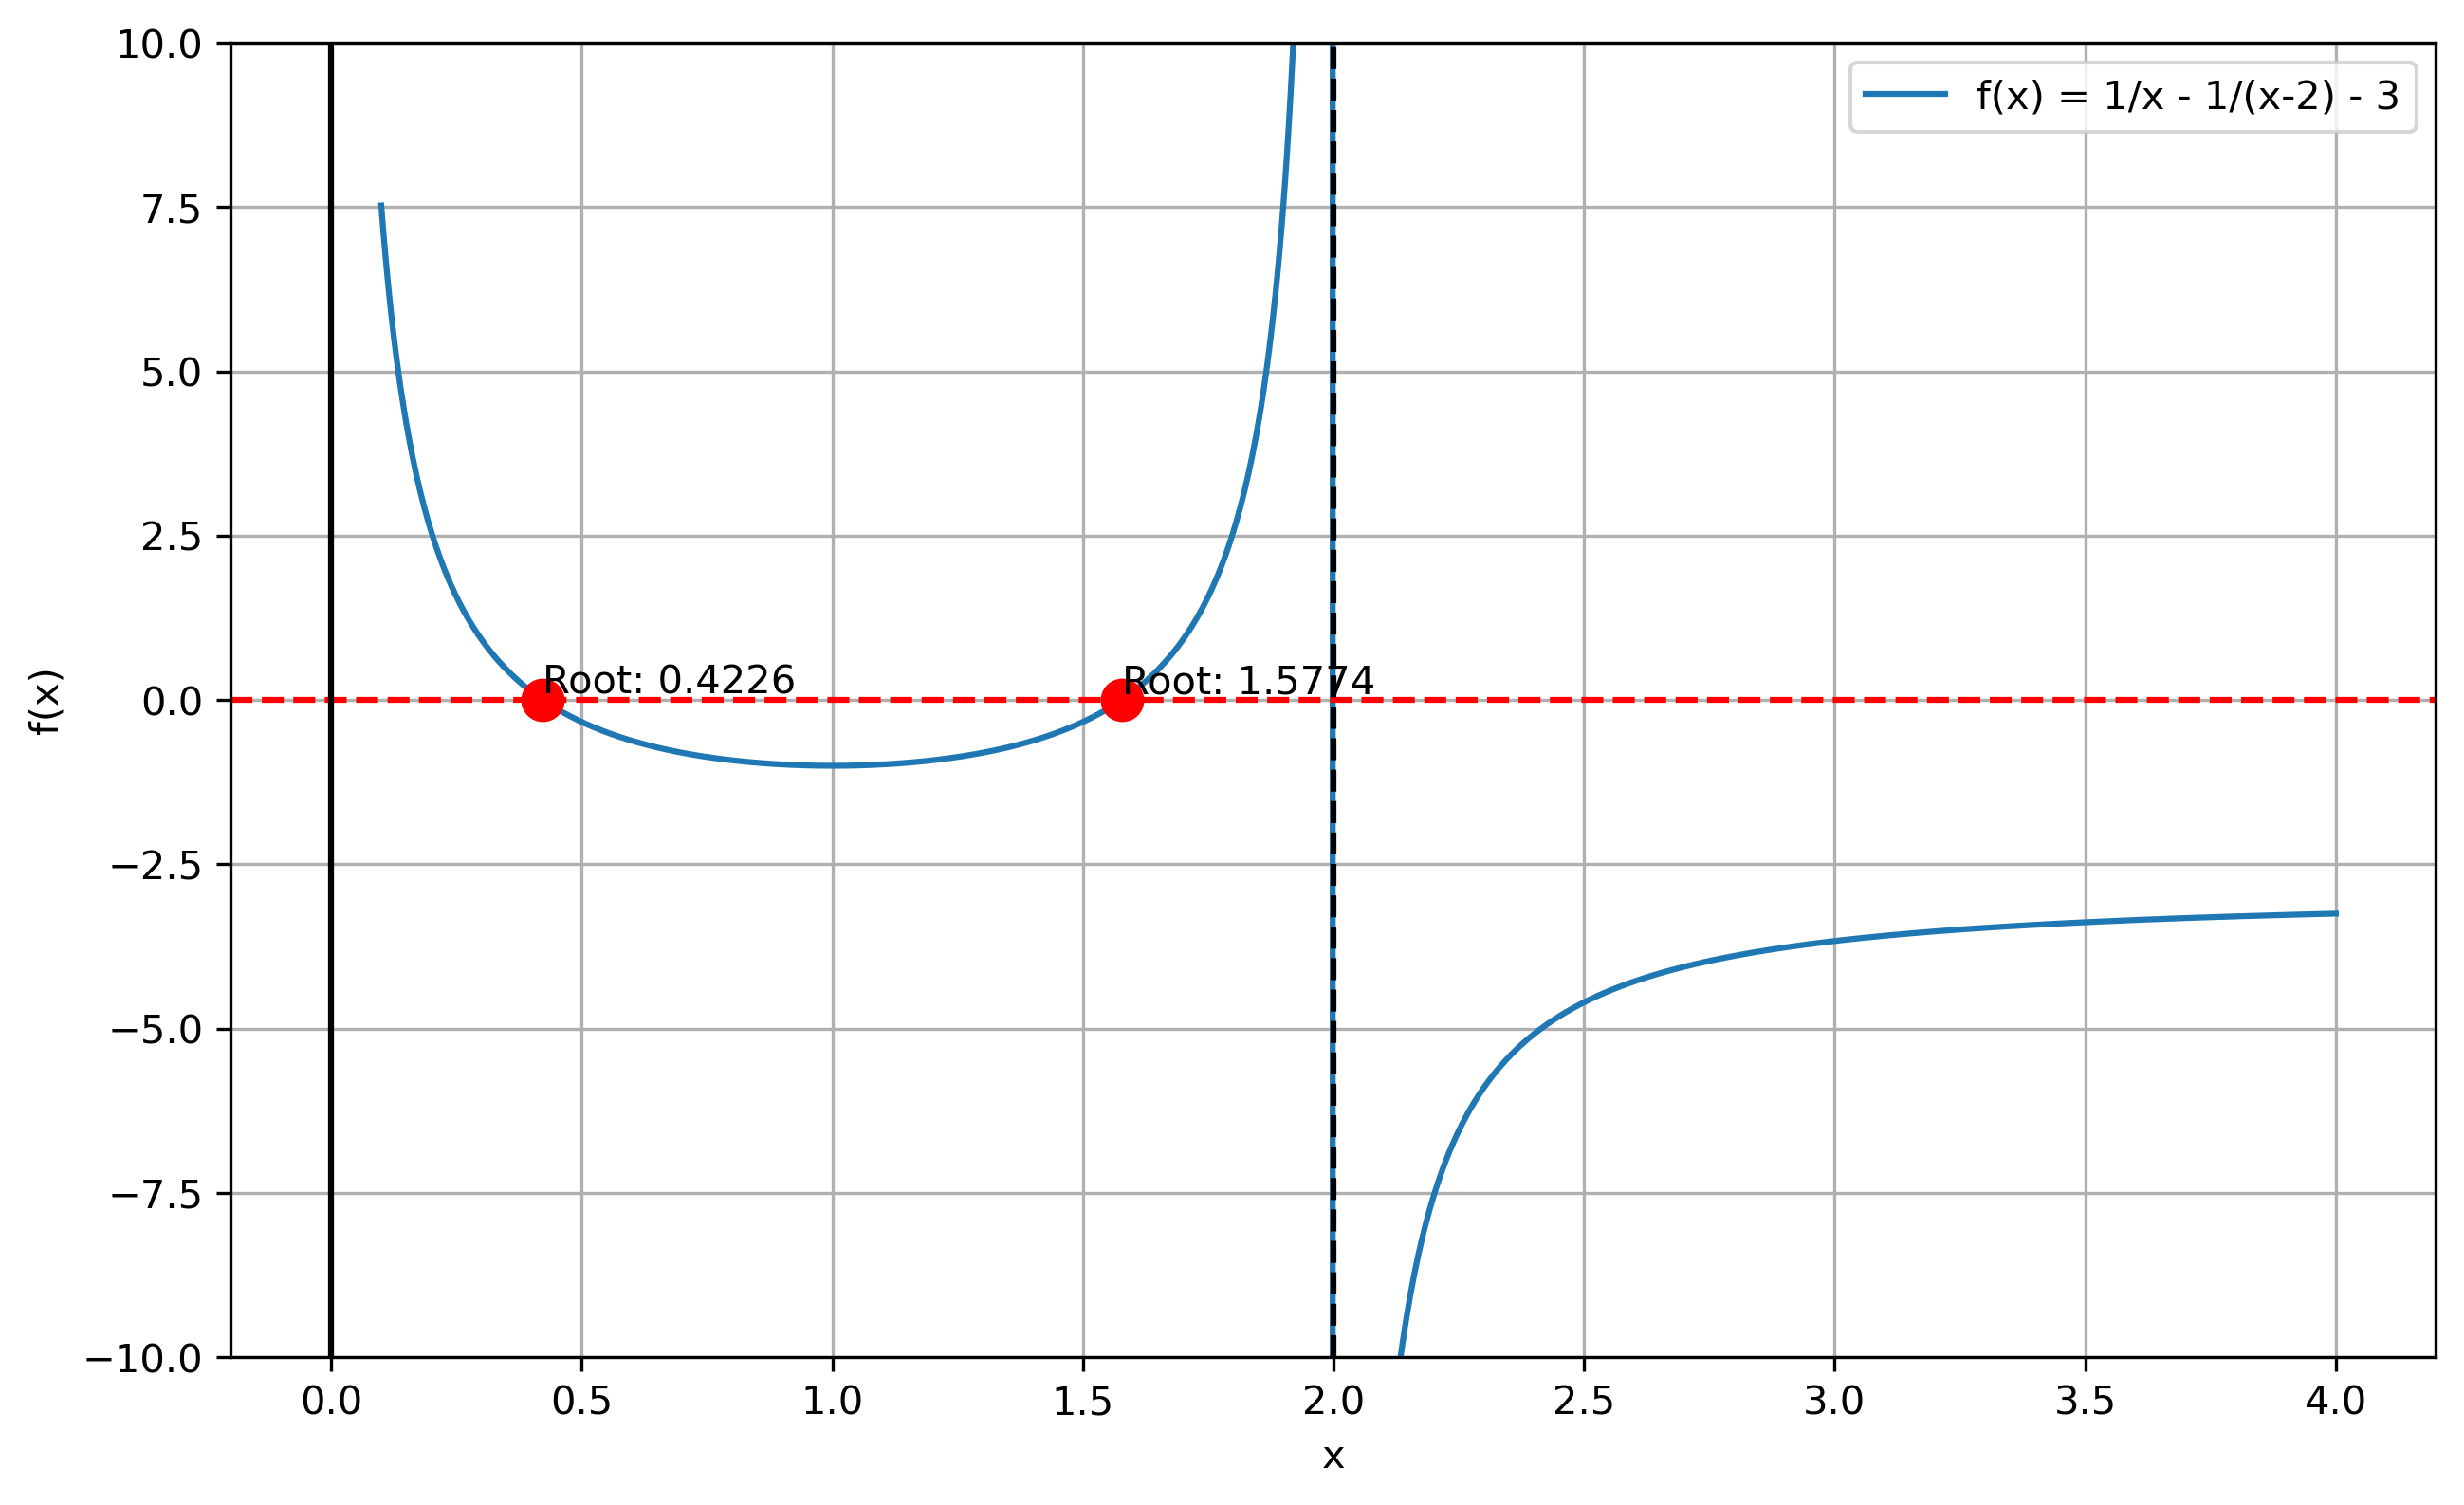
\includegraphics[width=\textwidth]{figs/fig.png}
\end{figure}
\end{document}
